\documentclass[compress,11 pt,t]{beamer}
\usetheme[
	bullet=circle,		% Other option: square
	bigpagenumber,		% circled page number on lower right
	topline=true,		% colored bar at the top of the frame 
	]{Zurich}
%\useoutertheme[subsection=false]{miniframes}  
\usepackage[utf8]{inputenc} % Required for inputting international characters
\usepackage{multicol}

%-----------------------------------------------------------------------------
% BEAMER TEMPLATE
\setbeamertemplate{section in toc}[sections numbered]
\setbeamerfont{subsection in toc}{size=\small}
\usepackage{etoolbox}
\makeatletter
\patchcmd{\slideentry}{\advance\beamer@xpos by1\relax}{}{}{}
\def\beamer@subsectionentry#1#2#3#4#5{\advance\beamer@xpos by1\relax}%
\makeatother


%-----------------------------------------------------------------------------
% DOCUMENT PROPERTIES

\author[\textsc{Oriol Colomés Gené}]{\emph{author:}\\
\textsc{Oriol Colomés Gené}\\[0.2cm]
\emph{supervisor:}\\
\textsc{Santiago Badia}}
\title[Large scale FE solvers for LES of incomprssible turbulent flows]{Large scale Finite Element solvers for the large eddy simulation of incompressible turbulent flows}
\institute{Departament d'Enginyeria Civil i Ambiental}
\titlegraphic{
\includegraphics[width=0.5\textwidth]{../../sources/Figures/Cover/logo_escola_pantone_201_C}}
%\titlegraphic{
\includegraphics[width=0.7\texwidth]{../../sources/Figures/Cover/logo_escola_pantone_201_C.png}}

%-----------------------------------------------------------------------------
%----------------------------------------------------------------------------------------
%	DEFINE CUSTOM SYMBOL COMMANDS
%----------------------------------------------------------------------------------------

% Bold
\def\u{{\bf u}}
\def\x{{\bf x}}
\def\r{{\bf r}}
\def\e{{\bf e}}
\def\a{{\bf a}}
\def\v{{\bf v}}
\def\w{{\bf w}}
\def\f{{\bf f}}
\def\n{{\bf n}}
\def\t{{\bf t}}
\def\k{{\bf k}}
\def\R{{\bf R}}
\def\F{{\bf F}}
\def\U{{\bf U}}
\def\P{{\bf P}}
\def\X{{\bf X}}
\def\H{\bf{H}}
\def\Lbf{{\bf L}}
\def\Hbf{{\bf H}}
\def\Tbf{{\bf T}}
\def\Cbf{{\bf C}}
\def\Rbf{{\bf R}}
\def\boldI{\mathbf{I}}

% Bold symbols
\def\XI{{\boldsymbol{\Xi}}}
\def\kppa{\boldsymbol{\kappa}}
\def\etaa{\boldsymbol{\eta}}
\def\xii{\boldsymbol{\xi}}
\def\KA{\boldsymbol{\Kappa}}
\def\ETA{\boldsymbol{\Upsilon}}
\def\boldsigma{\boldsymbol{\sigma}}
\def\boldomega{\boldsymbol{\omega}}
\def\boldzeta{\boldsymbol{\zeta}}

%Caligraphic
\def\Dcal{\mathcal{D}}
\def\Ccal{\mathcal{C}}

% BB
\def\M{\mathbb{M}}
\def\K{\mathbb{K}}
\def\C{\mathbb{C}}
\def\G{\mathbb{G}}
\def\D{\mathbb{D}}
\def\L{\mathbb{L}}
\def\A{\mathbb{A}}
\def\B{\mathbb{B}}
\def\I{\mathbb{I}}
\def\Sb{\mathbb{S}}
\def\Kt{\tilde{\mathbb{K}}}
\def\Bt{\tilde{\mathbb{B}}}
\def\Mt{\tilde{\mathbb{M}}}
\def\St{\tilde{\mathbb{S}}}
\def\At{\tilde{\mathbb{A}}}
\def\T{\mathbb{T}}
\def\Rbb{\mathbb{R}}

% Other
\def\half{\frac{1}{2}}
\def\Eq#1{(\ref{eq-#1})}
\def\Lem#1{\ref{lem-#1}}
\def\Fig#1{Figure \ref{fig-#1}}
\def\Chap#1{Chapter \ref{chap-#1}}
\def\Sec#1{Section \ref{sec-#1}}
\def\cl{ \nonumber \\}
\def\el{\nonumber}
\def\jumpl{\lbrack\!\lbrack}
\def\jumpr{\rbrack\!\rbrack}
\def\jump#1{\jumpl #1 \jumpr}
\def\jumpt#1{\underline{\jump{#1}}}
\def\mean#1{\{\! \!\{ #1\}\! \!\}}
\def\meanpv#1{\{ #1\}}
\def\meanhar#1{\langle#1\rangle}
\def\Qq{ \Omega \times (0,t^*)}

% New commands
\newtheorem{remark}{Remark}[section]
\newtheorem{proposition}{Proposition}[section]
\newcommand{\tickYes}{\checkmark}
\newcommand{\tickNo}{\hspace{1pt}\ding{55}}
\definecolor{tableShade}{HTML}{F1F5FA}



\begin{document}

%=========================================================================================
% TITLE
% ----------------------------------------------------------------------------
\addtocounter{framenumber}{-1}
\frame{\titlepage}
% ----------------------------------------------------------------------------
\addtocounter{framenumber}{-1}
\frame{\vfill\tableofcontents[subsectionstyle=hide,subsubsectionstyle=hide]\vfill}

%=========================================================================================
% 1.MOTIVATION
% ----------------------------------------------------------------------------
\section{Motivation}
\addtocounter{framenumber}{-1}
\frame{\vfill
	\tableofcontents[currentsection,
		 			  subsubsectionstyle=hide,						  sectionstyle=show/shaded, 
					  subsectionstyle=show/hide]
					  \vfill
}
\begin{frame}
\frametitle{Motivation}
\vfill
{\bf Thesis motivation }\\
\begin{itemize}
\item<2-> Turbulence is a very challenging problem:
\begin{itemize}
\item Many industrial applications
\item Understanding the phenomena (physics)
\end{itemize}
\item<3-> Computational Fluid Dynamics (CFD) to simulate such flows
\item<4-> Take advantage of increasing computational capacity (High-performance Computing (HPC))
\item<5-> In a Finite Element (FE) framework
\end{itemize}
\vfill
\end{frame}
%=========================================================================================
\begin{frame}
\frametitle{Objective}
\vfill
{\bf Thesis goal }\\
Highly scalable Finite Element (FE) framework for Large Eddy Simulations (LES) of incompressible turbulent flows\\
\vspace{0.5cm}
\onslide<2->{{\bf How to get there?}
\begin{enumerate}
\onslide<3->{\item \alert<3>{Variational MultiScale} (VMS) methods as LES models}
\onslide<4->{\item Time integration schemes with \alert<4>{velocity-pressure segregation}}
\onslide<5->{\item Highly scalable algorithms based on \alert<5>{Domain Decomposition (DD) and block preconditioners}}
\end{enumerate}}
\vfill
\end{frame}
%=========================================================================================
\begin{frame}
\frametitle{Objective}
\vfill
\textbf{Step by step...}
\begin{itemize}
\onslide<1->{\alert<6>{\item Residual-based VMS as LES models}}
\onslide<2->{\item Mixed FE formulations as LES models}
\onslide<3->{\item High-order time integration schemes}
\onslide<4->{\item Velocity-pressure segregation}
\onslide<5->{\item Scalable solvers}
\end{itemize}
\vfill
\end{frame}

%=========================================================================================
% 2.RESIDUAL-BASED VMS
% ----------------------------------------------------------------------------
\section{Residual-based VMS}
\addtocounter{framenumber}{-1}
\frame{
\begin{minipage}[\textheight]{0.5\textwidth}
\vfill
\tableofcontents[currentsection,
				subsubsectionstyle=hide,
				sectionstyle=show/shaded, 
				subsectionstyle=show/show/hide]
\vfill
\end{minipage}
\begin{minipage}[\textheight]{0.4\textwidth}
	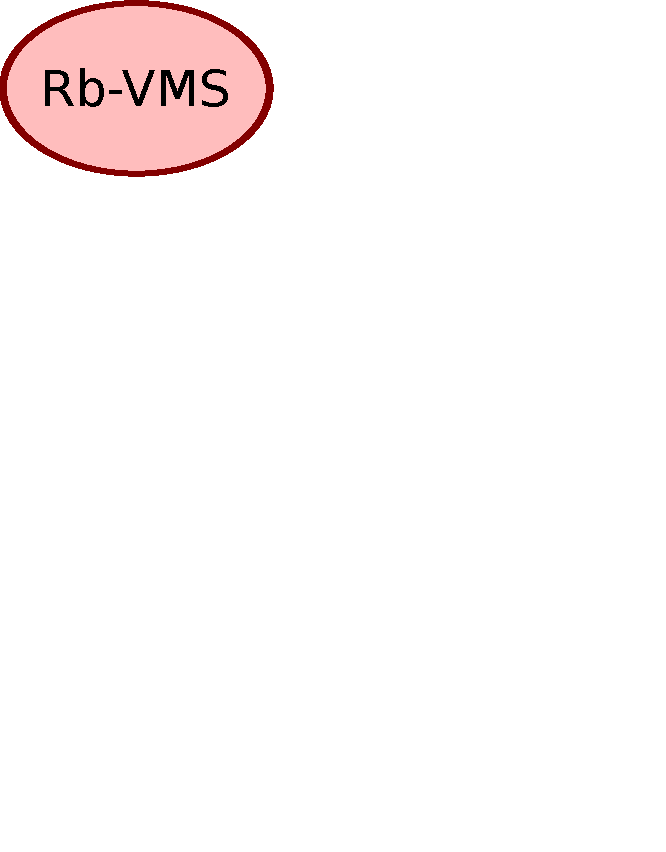
\includegraphics[width=1.1\textwidth]{Figures/index_1}
\end{minipage}
}
\begin{frame}
\frametitle{Implicit LES}
\vfill
\textbf{ILES}: only numerical dissipation (for stabilization) acts as turbulent model
\begin{overprint}
\onslide<1>
\begin{itemize}
\item Not based on filtering of the Navier-Stokes equations
\item Rely on numerical artifacts, no modification at the continuous level
\end{itemize}
\end{overprint}
\vfill
\end{frame}

%=========================================================================================
% 2.1.FORMULATION
% ----------------------------------------------------------------------------
\subsection{Formulation}
%----------------------------------------------------------------------------------------
\begin{frame}[t]
\frametitle{Incomp. Navier Stokes equations}
Find $ \mathbf{u}$ and $p$ defined in $\Omega$
\begin{align*}
\partial _{t}\mathbf{u}+ {\color<4>{red} \mathbf{u}\cdot \mathbf{\nabla u} }+\mathbf{
\nabla }p-\nu \nabla ^{2}\mathbf{u}& =\mathbf{f} \\
\mathbf{\nabla }\cdot \mathbf{u}& =0
\end{align*}
with appropriate boundary conditions on $ \Gamma$.\vskip 0.3cm
\only<2->{
The weak problem is: $\forall \mathbf{v}\in \mathcal{V}_0$ and  $\forall q\in \mathcal{Q}_0$, 
find $ \mathbf{u} \in \mathcal{V}$ and $ p \in \mathcal{Q}$ such that 
\begin{align*}
  \left( \mathbf{v},\partial_{t}\mathbf{u}\right)_{\Omega }
+ \left( \mathbf{\nabla v}, \nu \mathbf{\nabla u}\right)_{\Omega }  
%+ {\color<4>{red} \langle \mathbf{v},\mathbf{a}\cdot \mathbf{\nabla u}\rangle _{\Omega }} 
+ {\color<4>{red} b\left(\mathbf{u},\mathbf{u}, \mathbf{v}\right)} % \\
- \left( \mathbf{\nabla }\cdot \mathbf{v},p\right) _{\Omega } 
& = 
\left\langle \mathbf{v},\mathbf{f} \right\rangle _{\Omega } 
\\
\left(q, \mathbf{\nabla } \cdot \mathbf{u}\right)_{\Omega } 
& = 0
\end{align*}}
\only<3->{where
\begin{equation*}
{\color<4>{red} 
b\left(\mathbf{a},\mathbf{u}, \mathbf{v}\right) = {\color<1-3>{white} \frac{1}{2}}\langle \mathbf{v},\mathbf{a}\cdot \mathbf{\nabla u}\rangle_{\Omega }
{\color<1-3>{white} - \frac{1}{2} \langle \mathbf{a}\cdot\mathbf{\nabla}\mathbf{v}, \mathbf{u}\rangle_{\Omega }
+ \frac{1}{2} \langle \mathbf{v},\mathbf{n} \cdot \mathbf{a}  \mathbf{u} \rangle_{\Gamma }}}
\end{equation*}
}
\end{frame}
%----------------------------------------------------------------------------------------
\begin{frame}[t]
\frametitle{VMS decomposition {\small (Hughes 1995)}}
A decomposition of spaces $\mathcal{V}$ and $\mathcal{Q}$ given by 
\begin{equation*}
\mathcal{V}=\mathcal{V}_{h}\oplus \widetilde{\mathcal{V}},\quad
\mathcal{Q}=\mathcal{Q}_{h}\oplus \widetilde{\mathcal{Q}}
\end{equation*}
\only<2->{is applied to the function and test spaces
\begin{align*}
\mathbf{u} = \mathbf{u}_{h} +\widetilde{\mathbf{u}}, \quad p = p_h + \widetilde{p} \\
\mathbf{v} = \mathbf{v}_{h} +\widetilde{\mathbf{v}}, \quad q = q_h + \widetilde{q}
\end{align*}}
\only<3->{We keep all the (eight) contributions from the splitting of the convective
term 
\begin{equation*}
  { \mathbf{u}} \cdot \mathbf{\nabla u}
= { \mathbf{u}_{h}\cdot \mathbf{\nabla u}_{h} }
+ { \color<3->{red} \widetilde{\mathbf{u}}\cdot \mathbf{\nabla u}_{h} }
+ { \mathbf{u}_{h}\cdot \mathbf{\nabla }\widetilde{\mathbf{u}} }
+ { \color<3->{red} \widetilde{\mathbf{u}}\cdot \mathbf{\nabla }\widetilde{\mathbf{u}} }
\end{equation*}
}
\only<4->{and all the (four) contributions from the temporal term 
\begin{equation*}
\partial _{t}\mathbf{u}=\partial _{t}\mathbf{u}_{h} + { \color<4->{red} \partial _{t}\widetilde{\mathbf{u}}}
\end{equation*}
}
\end{frame}
%----------------------------------------------------------------------------------------
\begin{frame}[t]
\frametitle{Semidiscrete problem}
\begin{block}{FEM equations}
\begin{overlayarea}{\textwidth}{2.0cm}
\vspace{-0.8cm}
\begin{align*}
% FEM EQUATIONS
\only<1>{B\left(\left(\mathbf{u}_h,p_h\right);\left(\widetilde{\mathbf{u}},\widetilde{p}\right);\left(\mathbf{v}_h,q_h\right)\right)=L\left(\mathbf{v}_h,q_h\right)}
\only<2->{\left( \mathbf{v}_{h},\partial _{t}\mathbf{u}_{h}\right) _{\Omega }
%+\langle \mathbf{v}_{h},\mathbf{a}\cdot \mathbf{\nabla u}_{h}\rangle _{\Omega}
+ b\left(\mathbf{a},\mathbf{u}_h, \mathbf{v}_h\right)
+\left( \mathbf{\nabla v}_{h},\nu \mathbf{\nabla u}_{h}\right) _{\Omega} &
-\left( \mathbf{\nabla }\cdot \mathbf{v}_{h},p_{h}\right) _{\Omega }
\\[0.05in]
%
+\left( \mathbf{v}_{h},\partial _{t}\widetilde{\mathbf{u}}\right) _{\Omega}
+\left( \mathcal{L}^{\ast }\mathbf{v}_{h},\widetilde{\mathbf{u}}\right)_{\Omega^h}
-\left( \mathbf{\nabla }\cdot \mathbf{v}_{h},\widetilde{p}\right) _{\Omega^h} &
=\left\langle \mathbf{v}_{h},\mathbf{f}\right\rangle_{\Omega }
\\[0.1in]
%
\left( q_{h},\mathbf{\nabla }\cdot \mathbf{u}_{h}\right) _{\Omega }
-\left( \mathbf{\nabla }q_{h},\widetilde{\mathbf{u}}\right) _{\Omega^h} & =0}
\end{align*}
\end{overlayarea}
\end{block}
\begin{block}{SGS equations}
\vspace{-0.4cm}
\begin{align*}
% SGS EQUATIONS
\only<1>{B\left(\left(\widetilde{\mathbf{u}},\widetilde{p}\right);\left(\mathbf{u}_h,p_h\right);\left(\widetilde{\mathbf{v}},\widetilde{q}\right)\right)=L\left(\widetilde{\mathbf{v}},\widetilde{q}\right)}
%\only<1-4>{\left( \widetilde{\mathbf{v}},\partial_{t} \widetilde{\mathbf{u}} \right)_{\Omega }}
%\only<1-2>{\color<2>{red}  + \left( \widetilde{\mathbf{v}},\mathcal{L}\widetilde{\mathbf{u}}\right )_{\Omega^h}}
%\only<3-4>{\color<3>{red}  + \tau _{m}^{-1} \left( \widetilde{\mathbf{v}},\widetilde{\mathbf{u}} \right)_{\Omega^h}}
%\only<1-2>{\color<2>{blue} + \left( \widetilde{\mathbf{v}},\mathbf{\nabla }\widetilde{p}\right)_{\Omega^h} }
%%\only<1-4>{\color{white}\tau _{m}^{-1}} % This is needed to avoid a vertical blinking 
\only<2-> {{\color<5>{red} \partial_{t}\widetilde{\mathbf{u}}} + {\color<2>{red}\tau_{m}^{-1}} \widetilde{\mathbf{u}}}
&
\only<2-> { = {\color<4>{red}\mathcal{P}} {\color<3>{red}\mathbf{R}_{m} }}
\only<1>{\\[0.05in]}
%
%\only<1->{{ \color{white}\tau_{c}^{-1} }}
%\only<1-4>{ \color<4>{red}
%+\left( \widetilde{\mathbf{v}},\partial _{t}\mathbf{u}_{h}\right)_{\Omega}
%+\left( \widetilde{\mathbf{v}},\mathcal{L}\mathbf{u}_{h}\right)_{\Omega^h}
%+\left( \widetilde{\mathbf{v}},\mathbf{\nabla }p_{h}\right)_{\Omega^h}
%& = 
%\color<4>{red} \left\langle \widetilde{\mathbf{v}},\mathbf{f}\right\rangle _{\Omega} }
%%
\\[0.1in]
%%
%%\only<1->{{ \color{white}\tau_{c}^{-1} }}
%\only<1-2>{{\color<2>{blue} \left(( \widetilde{q},\mathbf{\nabla} \cdot \widetilde{\mathbf{u}}\right)_{\Omega }}}
%\only<3-4>{{\color<3>{blue} \tau_{c}^{-1} \left( \widetilde{q},\widetilde{p}\right) _{\Omega^h }}}
%\only<1-4>{ + {\color<4>{blue} \left( \widetilde{q},\mathbf{\nabla}\cdot \mathbf{u}_{h}\right)_{\Omega } }} 
%\only<1-4>{& = 0}
\only<2->{ {\color<2>{blue} \tau _{c}^{-1}} \widetilde{p} & = {\color<4>{blue}\mathcal{P}} {\color<3>{blue}R_{c}}}
\end{align*}
\end{block}
%\end{overlayarea}
\vspace{-0.2cm}
\begin{overlayarea}{\textwidth}{3.0cm}
\only<1>{
\vspace*{-1.0cm}
\begin{equation*}
%\mathcal{L}=-\nu \nabla ^{2}+\mathbf{a}\cdot \mathbf{\nabla },\quad 
%\mathcal{L}^{\ast }=-\nu \nabla ^{2}-\mathbf{a}\cdot \mathbf{\nabla },\quad
%\mathbf{a=u}_{h}+\widetilde{\mathbf{u}}
\end{equation*}
}
\only<2>{
\begin{equation*}
{ \color<2>{red} \tau_{m}=\left( \frac{c_{1}\nu }{h^{2}}+\frac{c_{2}\left| \mathbf{a}\right| }{h}\right) ^{-1}},\quad
{ \color<2>{blue}\tau_{c}=\frac{h^{2}}{c_{1}\tau _{m}} }
\end{equation*}
}
\only<3>{
\begin{equation*}
{ \color<3>{red} \mathbf{R}_{m}} := \mathbf{f} - \partial_{t}\mathbf{u}_{h} - \mathcal{L} \mathbf{u}_{h} - \mathbf{\nabla }p_{h}, \quad
{ \color<3>{blue} R_{c}} := - \mathbf{\nabla }\cdot \mathbf{u}_{h}
\end{equation*}
}
\only<4->{
\begin{equation*}
\only<4>{{\color<4>{red} \mathcal{P} = I \quad \rm{(ASGS)}}, \quad \quad {\color<4>{blue} \mathcal{P} = P_h^{\perp}=I-P_h \quad \rm{(OSS)}} }
\only<5->{{\color<5>{magenta} \mathcal{P} = I \quad \rm{(ASGS)}, \quad \quad  \mathcal{P} = P_h^{\perp}=I-P_h \quad \rm{(OSS)} }}
\end{equation*}
}
\only<2,5>{
\vspace{-0.2cm}
\begin{equation*}
{\color<5>{blue} \mathbf{a=u}_{h}+\widetilde{\mathbf{u}} }
\end{equation*}
}
\end{overlayarea}
%
%\begin{overlayarea}{\textwidth}{1.5cm}
%%\only<3->{
%\begin{equation*}
%{\color<6>{blue} \mathbf{a=u}_{h}+\widetilde{\mathbf{u}}} 
%{\color<1-2>{white}, \quad \tau_{m}=\left(( \frac{c_{1}\nu }{h^{2}}+\frac{c_{2}\left| \mathbf{a}\right| }{h}\right) ^{-1},\quad
%\tau_{c}=\frac{h^{2}}{c_{1}\tau _{m}} }
%\end{equation*}
%%}
%\end{overlayarea}
\end{frame}


%=========================================================================================
% 2.2.ENERGY STATEMENTS
% ----------------------------------------------------------------------------
\subsection{Energy statements}
\begin{frame}[t]
\frametitle{Energy statements}
\begin{overlayarea}{\textwidth}{0.25\textheight}
\textbf{FE counterpart:}
\vspace*{-0.3cm}
\only<1>{
\begin{align*}
&B\left(\left(\mathbf{u}_h,p_h\right);\left(\widetilde{\mathbf{u}},\widetilde{p}\right);\left(\mathbf{u}_h,p_h\right)\right)=L\left(\mathbf{u}_h,p_h\right)
\end{align*}}
\only<2->{
\begin{align*}
&\alert<3>{\frac{1}{2}d_t\|\u_h\|^2}+\alert<4>{\nu\|\nabla\u_h\|^2}+\alert<5>{b(\a,\u_h,\u_h)}\\
&\alert<7>{+\left( \partial _{t}\widetilde{\u},\u_{h}\right)
+\left( \mathcal{L}^{\ast }_a(\u_{h},p_h),\widetilde{\u}\right)
-\left( \mathbf{\nabla }\cdot \u_{h},\widetilde{p}\right)}
=\alert<8>{\left\langle \mathbf{f},\u_{h}\right\rangle}
\end{align*}}
\end{overlayarea}
\begin{overlayarea}{\textwidth}{0.25\textheight}
\textbf{SGS counterpart:}
\vspace*{-0.3cm}
\only<1>{
\begin{align*}
&B\left(\left(\widetilde{\mathbf{u}},\widetilde{p}\right);\left(\mathbf{u}_h,p_h\right);\left(\widetilde{\mathbf{u}},\widetilde{p}\right)\right)=L\left(\widetilde{\mathbf{u}},\widetilde{p}\right)
\end{align*}}
\only<2->{
\begin{align*}
&\alert<3>{\frac{1}{2}d_t\|\widetilde{\u}\|^2}\alert<6>{+\tau_m^{-1}\|\widetilde{\u}\|^2+\tau_c^{-1}\|\widetilde{p}\|^2}\\
&\alert<7>{+\left( \mathcal{P}(\partial _{t}\u_{h}),\widetilde{\u}\right)
+\left( \mathcal{P}(\mathcal{L}^{\ast }_a(\u_{h},p_h)),\widetilde{\u}\right)
-\left( \mathcal{P}(\mathbf{\nabla }\cdot \u_{h}),\widetilde{p}\right)}
=\alert<8>{\left\langle \mathcal{P}(\mathbf{f}),\widetilde{\u}\right\rangle}
\end{align*}}
\end{overlayarea}
\begin{overlayarea}{\textwidth}{0.5\textheight}
\textbf{TOTAL:}
\only<9>{\alert<9>{\textbf{ Static subscales}}}
\only<10->{\alert<10->{\textbf{ Dynamic subscales}}}
\only<10>{\alert<10>{\textbf{- ASGS}}}
\only<11>{\alert<11>{\textbf{- OSS}}}
\only<1>{
\begin{align*}
&B\left(\left(\mathbf{u}_h,p_h\right);\left(\widetilde{\mathbf{u}},\widetilde{p}\right);\left(\mathbf{u}_h,p_h\right)\right)\\
+&B\left(\left(\widetilde{\mathbf{u}},\widetilde{p}\right);\left(\mathbf{u}_h,p_h\right);\left(\widetilde{\mathbf{u}},\widetilde{p}\right)\right)=L\left(\mathbf{u}_h,p_h\right)+L\left(\widetilde{\mathbf{u}},\widetilde{p}\right)
\end{align*}}
\only<3-8>{
\begin{align*}
&\alert<3>{\frac{1}{2}d_t\|\u_h\|^2+\frac{1}{2}d_t\|\widetilde{\u}\|^2}
\onslide<4-8>{
\alert<4>{+\nu\|\nabla\u_h\|^2}
\onslide<6-8>{
\alert<6>{+\tau_m^{-1}\|\widetilde{\u}\|^2+\tau_c^{-1}\|\widetilde{p}\|^2}\\
\onslide<7-8>{
&\alert<7>{+\left( \partial _{t}\widetilde{\u},\u_{h}\right)+\left( \mathcal{P}(\partial _{t}\u_{h}),\widetilde{\u}\right)
+\left( \mathcal{L}^{\ast }_a(\u_{h},p_h),\widetilde{\u}\right)+\left( \mathcal{P}(\mathcal{L}^{\ast }_a(\u_{h},p_h)),\widetilde{\u}\right)}\\
&\alert<7>{
-\left( \mathbf{\nabla }\cdot \u_{h},\widetilde{p}\right)
-\left( \mathcal{P}(\mathbf{\nabla }\cdot \u_{h}),\widetilde{p}\right)}
\onslide<8>{
=\alert<8>{\left\langle \mathbf{f},\u_{h}\right\rangle+\left\langle \mathcal{P}(\mathbf{f}),\widetilde{\u}\right\rangle}
}}}}
\end{align*}}
\only<9->{
\begin{align*}
&\only<9,11>{\frac{1}{2}d_t\|\u_h\|^2}
\only<10>{\frac{1}{2}d_t\|\u_h+\widetilde{\u}\|^2}
\onslide<11>{+\frac{1}{2}d_t\|\widetilde{\u}\|^2}
+\nu\|\nabla\u_h\|^2
+\tau_m^{-1}\|\widetilde{\u}\|^2+\tau_c^{-1}\|\widetilde{p}\|^2\\
&\only<9>{\onslide<11>{+\left( \partial _{t}\widetilde{\u},\u_{h}\right)}+\left( \mathcal{P}(\partial _{t}\u_{h}),\widetilde{\u}\right)
+\left( \mathcal{L}^{\ast }_a(\u_{h},p_h),\widetilde{\u}\right)+\left( \mathcal{P}(\mathcal{L}^{\ast }_a(\u_{h},p_h)),\widetilde{\u}\right)}
\only<10,11>{-2\left( \nu\Delta\u_h,\widetilde{\u}\right)}\\
&\onslide<9>{-\left( \mathbf{\nabla }\cdot \u_{h},\widetilde{p}\right)
-\left( \mathcal{P}(\mathbf{\nabla }\cdot \u_{h}),\widetilde{p}\right)}
=\left\langle \mathbf{f},\u_{h}\right\rangle
\only<9,11>{+\left\langle \mathcal{P}(\mathbf{f}),\widetilde{\u}\right\rangle}
\only<10>{+\left\langle \mathbf{f},\widetilde{\u}\right\rangle}
\end{align*}}
\end{overlayarea}

\end{frame}

%=========================================================================================
% 2.3.NUMERICAL EXPERIMENTS
% ----------------------------------------------------------------------------
\subsection{Numerical experiments}

%=========================================================================================
% 2.3.1.DHIT
% ----------------------------------------------------------------------------
\subsubsection{DHIT}

%=========================================================================================
% 2.3.2.TGV
% ----------------------------------------------------------------------------
\subsubsection{TGV}

%=========================================================================================
% 2.3.3.TCF
% ----------------------------------------------------------------------------
\subsubsection{TCF}

%=========================================================================================
% 2.4.CONCLUSIONS
% ----------------------------------------------------------------------------
\subsection{Conclusions}

%=========================================================================================
% 3.MIXED FE VMS
% ----------------------------------------------------------------------------
\section{Mixed FE VMS}
\addtocounter{framenumber}{-1}
\frame{
\begin{minipage}[\textheight]{0.5\textwidth}
\vfill
\tableofcontents[currentsection,
				subsubsectionstyle=hide,
				sectionstyle=show/shaded, 
				subsectionstyle=show/show/hide]
\vfill
\end{minipage}
\begin{minipage}[\textheight]{0.4\textwidth}
  	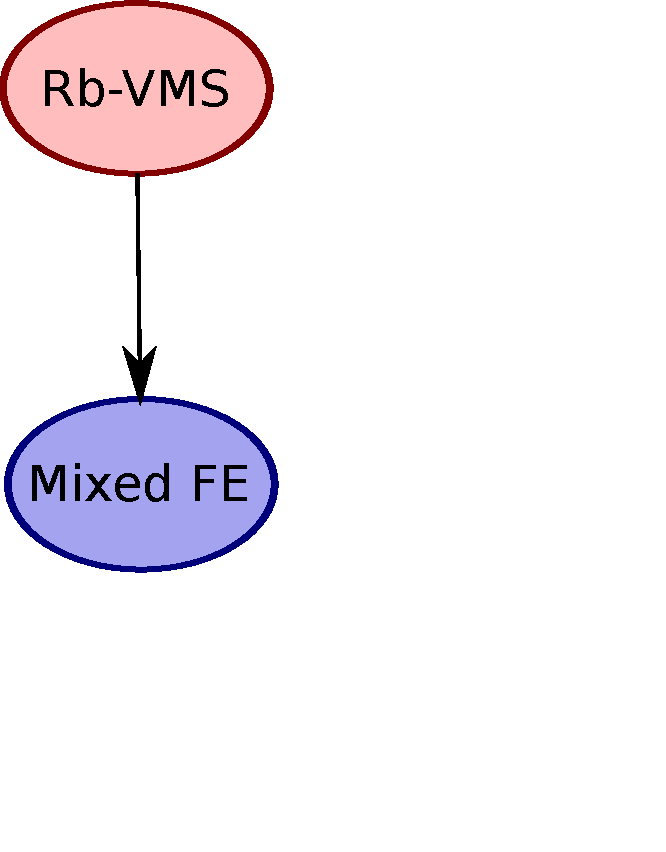
\includegraphics[width=1.1\textwidth]{Figures/index_2}
\end{minipage}
}

%=========================================================================================
% 3.1.FORMULATION
% ----------------------------------------------------------------------------
\subsection{Formulation}

%=========================================================================================
% 3.2.BLOCK-PRECONDITIONING
% ----------------------------------------------------------------------------
\subsection{Block-preconditioning}

%=========================================================================================
% 3.3.NUMERICAL EXPERIMENTS
% ----------------------------------------------------------------------------
\subsection{Numerical experiments}

%=========================================================================================
% 3.3.1.TGV
% ----------------------------------------------------------------------------
\subsubsection{TGV}

%=========================================================================================
% 3.3.2.TCF
% ----------------------------------------------------------------------------
\subsubsection{TCF}

%=========================================================================================
% 3.4.CONCLUSIONS
% ----------------------------------------------------------------------------
\subsection{Conclusions}

%=========================================================================================
% 4.SRK
% ----------------------------------------------------------------------------
\section{Segregated Runge-Kutta}
\addtocounter{framenumber}{-1}
\frame{
\begin{minipage}[\textheight]{0.5\textwidth}
\vfill
\tableofcontents[currentsection,
				subsubsectionstyle=hide,
				sectionstyle=show/shaded, 
				subsectionstyle=show/show/hide]
\vfill
\end{minipage}
\begin{minipage}[\textheight]{0.4\textwidth}
  	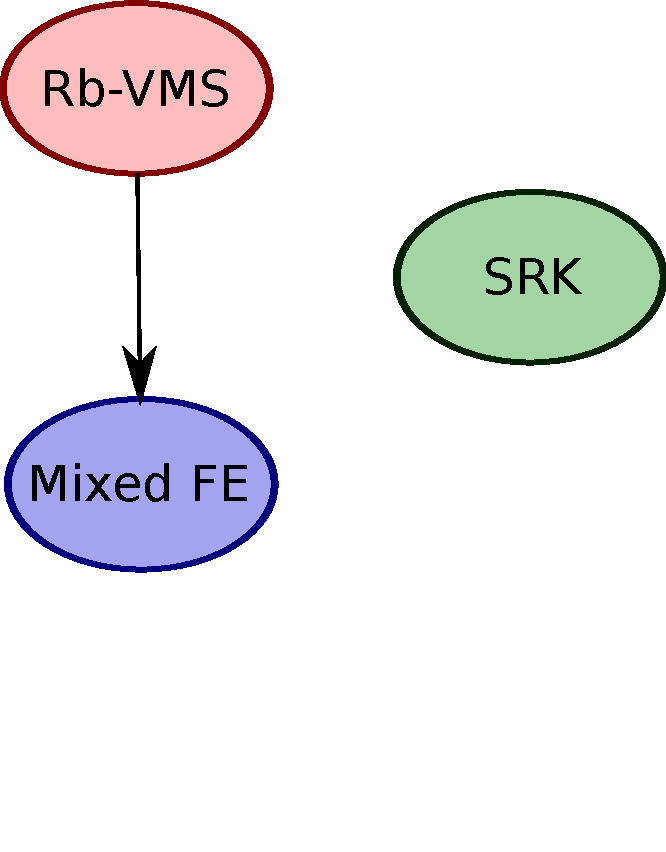
\includegraphics[width=1.1\textwidth]{Figures/index_3}
\end{minipage}
}

%=========================================================================================
% 4.1.FORMULATION
% ----------------------------------------------------------------------------
\subsection{Formulation}

%=========================================================================================
% 4.2.NUMERICAL EXPERIMENTS
% ----------------------------------------------------------------------------
\subsection{Numerical experiments}

%=========================================================================================
% 4.2.1.ANALYTICAL
% ----------------------------------------------------------------------------
\subsubsection{Analytical solution}

%=========================================================================================
% 4.2.2.CYLINDER
% ----------------------------------------------------------------------------
\subsubsection{Flow around a cylinder}

%=========================================================================================
% 4.3.CONCLUSIONS
% ----------------------------------------------------------------------------
\subsection{Conclusions}

%=========================================================================================
% 5.SVMS
% ----------------------------------------------------------------------------
\section{Segregated VMS}
\addtocounter{framenumber}{-1}
\frame{
\begin{minipage}[\textheight]{0.5\textwidth}
\vfill
\tableofcontents[currentsection,
			  	subsubsectionstyle=hide,
				sectionstyle=show/shaded, 
				subsectionstyle=show/show/hide]
\vfill
\end{minipage}
\begin{minipage}[\textheight]{0.4\textwidth}
  	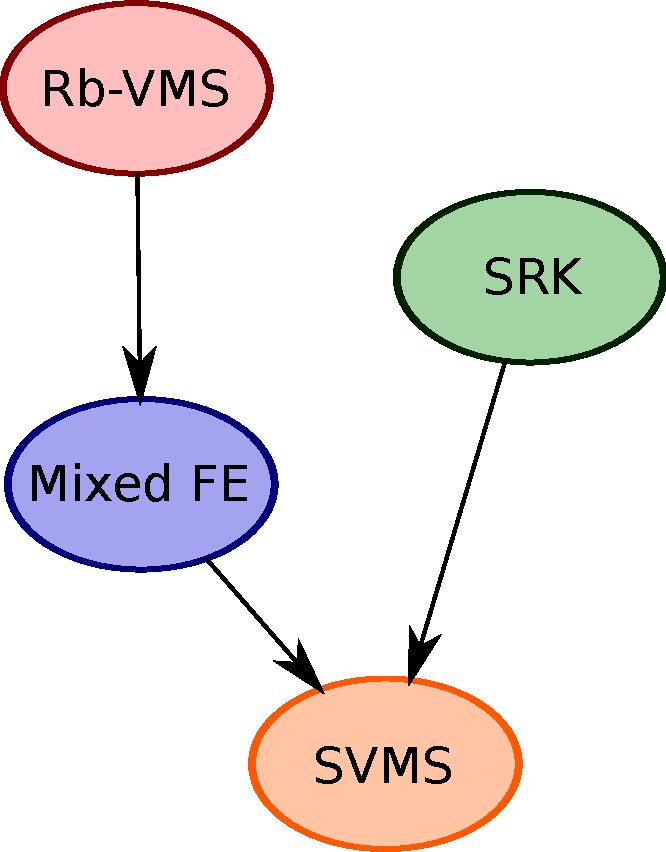
\includegraphics[width=1.1\textwidth]{Figures/index}
\end{minipage}
}

%=========================================================================================
% 5.1.FORMULATION
% ----------------------------------------------------------------------------
\subsection{Formulation}

%=========================================================================================
% 5.2.BLOCK-PRECONDITIONING
% ----------------------------------------------------------------------------
\subsection{Block-preconditioning}

%=========================================================================================
% 5.3.NUMERICAL EXPERIMENTS
% ----------------------------------------------------------------------------
\subsection{Numerical experiments}

%=========================================================================================
% 5.3.1.TGV
% ----------------------------------------------------------------------------
\subsubsection{TGV}

%=========================================================================================
% 5.3.2.TCF
% ----------------------------------------------------------------------------
\subsubsection{TCF}

%=========================================================================================
% 5.3.3.NACA
% ----------------------------------------------------------------------------
\subsubsection{Flow around a NACA profile}

%=========================================================================================
% 5.4.CONCLUSIONS
% ----------------------------------------------------------------------------
\subsection{Conclusions}

%=========================================================================================
% 6.CONCLUSIONS
% ----------------------------------------------------------------------------
\section{Conclusions}
\addtocounter{framenumber}{-1}
\frame{\vfill\tableofcontents[currentsection,
							  subsubsectionstyle=hide,
							  sectionstyle=show/shaded, 
							  subsectionstyle=show/show/hide]
}




\begin{frame}
\frametitle{Outline}
%\framesubtitle{Handwriting}

\begin{itemize}
    \item Line 1.
    \only<2->{
    \item Line 2.\\
        {\handwriting \textcolor{tangocolordarkchameleon}{Less formal} }
    }
    \only<3->{
    \item Line 3.\\
        {\handwriting \textcolor{tangocolordarkscarletred}{
        Less formal, different color.} }
    }
\end{itemize}


\end{frame}
% ----------------------------------------------------------------------------


% ----------------------------------------------------------------------------
\begin{frame}
\frametitle{Blocks}

\begin{block}{Standard Block}
    This is a standard block.
\end{block}

\begin{exampleblock}{Example Block}
    This is an example block.
\end{exampleblock}

\begin{alertblock}{Alert Block}
    This is an alert block.
\end{alertblock}



\end{frame}
% ----------------------------------------------------------------------------


% ----------------------------------------------------------------------------
\usebackgroundtemplate{
   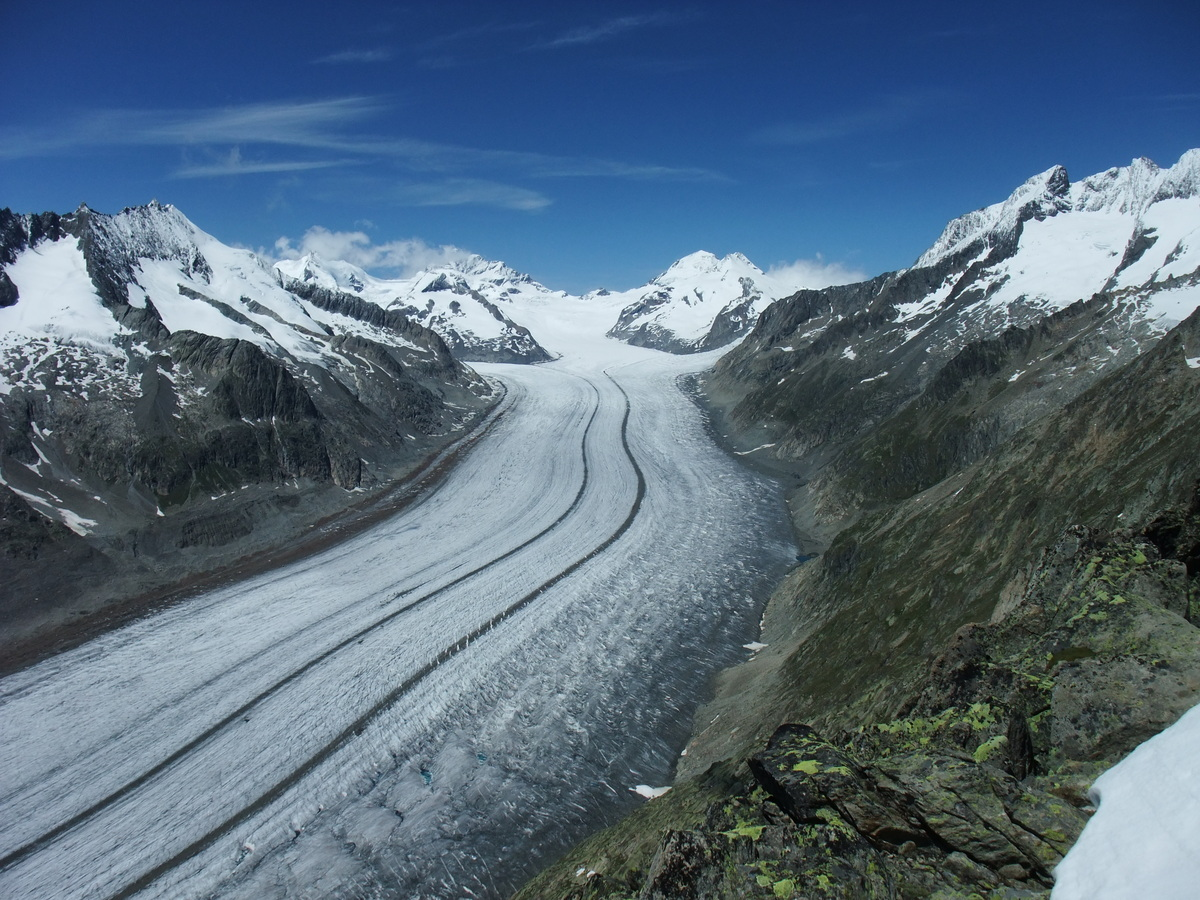
\includegraphics[width=\paperwidth,
                    height=\paperheight]{aletsch}
}
\begin{frame}
\ \\ \ \\
\centering \Large \textcolor{white}{Questions?}

\end{frame}
\usebackgroundtemplate{}
% ----------------------------------------------------------------------------


\end{document}
